The data were analyzed as static collection in order to facilitate
interpretation of the problems. Using a stream analysis many decision-making
for the allocation of resources might be misleading.
Figure~\ref{fig:rain_4_heat} shows an example for the keyword \emph{``rain''}.

\begin{figure}[!h]
    \centering
    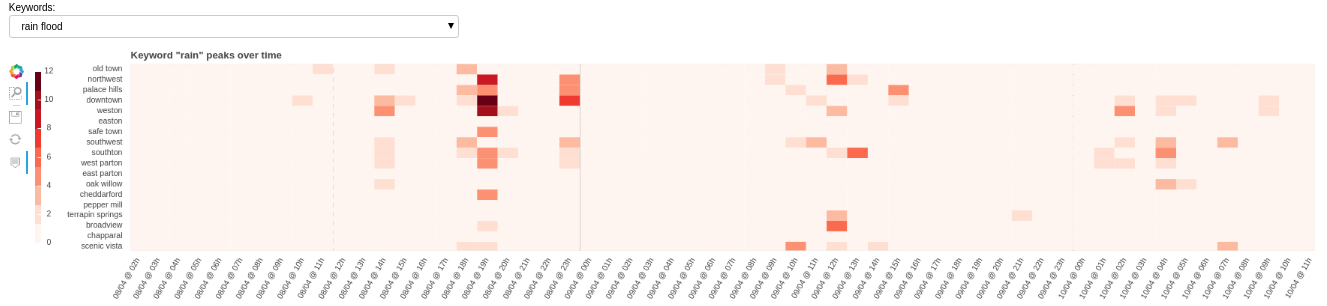
\includegraphics[width=1.00\textwidth]{figs/q4/rain_4_heat}
    \caption{Heatmap for the ``\emph{rain}''.}
    \label{fig:rain_4_heat}
\end{figure}

At 6:00 PM, five neighborhoods tweeted about rain or flood. If for each locality
a rescue team was sent, at 7:00 PM where almost all localities reported rain or
flood occurrences, so it would have been more difficult to efficiently serve all
those affected neighborhoods.
